\documentclass[border=4pt]{standalone}
% Paleta y fuentes compartidas por el libro y las figuras (única fuente de verdad).
\RequirePackage{xcolor}
\definecolor{oxido}{HTML}{B7410E}
\definecolor{cobre}{HTML}{D27D2D}
\definecolor{carbon}{HTML}{2B2B2B}
\definecolor{azul}{HTML}{1F5F8B}
\definecolor{arena}{HTML}{F4EDE4}

\usepackage{fontspec,pgfplots}
\pgfplotsset{compat=1.18}
\pgfkeys{/pgf/number format/assume math mode=true,/pgf/number format/use comma}
\setsansfont{FiraSans}[Extension=.otf,UprightFont=*-Regular,BoldFont=*-SemiBold,ItalicFont=*-Italic]
\begin{document}
\sffamily\small
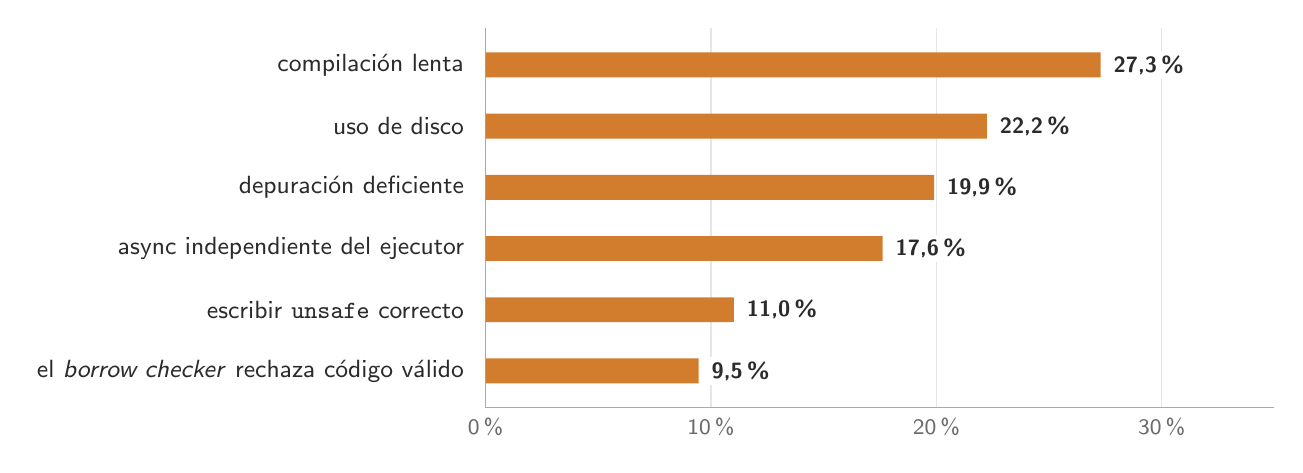
\begin{tikzpicture}
\begin{axis}[
  xbar, width=11.6cm, height=6.4cm, xmin=0, xmax=35, bar width=9pt,
  symbolic y coords={bc,uns,asy,dep,dis,comp}, ytick=data,
  yticklabels={el \textit{borrow checker} rechaza código válido,escribir \texttt{unsafe} correcto,async independiente del ejecutor,depuración deficiente,uso de disco,compilación lenta},
  y tick label style={font=\sffamily\small,text=carbon},
  xtick={0,10,20,30}, xticklabel={\pgfmathprintnumber{\tick}\,\%},
  x tick label style={font=\sffamily\footnotesize,text=carbon!70},
  axis x line*=bottom, axis y line*=left, axis line style={carbon!40},
  xmajorgrids, grid style={carbon!12}, tick style={draw=none},
  enlarge y limits=0.12, point meta=x,
  nodes near coords={\pgfmathprintnumber[fixed,fixed zerofill,precision=1]{\pgfplotspointmeta}\,\%},
  nodes near coords style={font=\sffamily\footnotesize\bfseries,text=carbon,anchor=west,xshift=3pt,fill=white,inner sep=1.5pt},
]
\addplot[fill=cobre,draw=none] coordinates {
  (9.45,bc) (11.02,uns) (17.62,asy) (19.90,dep) (22.24,dis) (27.29,comp)};
\end{axis}
\end{tikzpicture}
\end{document}
